\documentclass[12pt,a4paper]{article}
%\usepackage{ctex}
\usepackage{amsmath,amscd,amsbsy,amssymb,latexsym,url,bm,amsthm}
\usepackage{epsfig,graphicx,subfigure}
\usepackage{enumitem,balance}
\usepackage{wrapfig}
\usepackage{mathrsfs,euscript}
\usepackage[x11names,svgnames,dvipsnames]{xcolor}
\usepackage{hyperref}
\usepackage[vlined,ruled,commentsnumbered,linesnumbered]{algorithm2e}
\usepackage{listings}
\usepackage{multicol}


\usepackage{tikz}
\usepackage{verbatim}
%\usepackage[active,tightpage]{preview}
\usepackage{preview}
\PreviewEnvironment{tikzpicture}
\usetikzlibrary{trees}

\usepackage{fontspec}
\renewcommand{\listalgorithmcfname}{List of Algorithms}
\renewcommand{\algorithmcfname}{Alg}

\newtheorem{theorem}{Theorem}
\newtheorem{lemma}[theorem]{Lemma}
\newtheorem{proposition}[theorem]{Proposition}
\newtheorem{corollary}[theorem]{Corollary}
\newtheorem{exercise}{Exercise}
\newtheorem*{solution}{Solution}
\newtheorem{definition}{Definition}
\theoremstyle{definition}


%\numberwithin{equation}{section}
%\numberwithin{figure}{section}

\renewcommand{\thefootnote}{\fnsymbol{footnote}}

\newcommand{\postscript}[2]
 {\setlength{\epsfxsize}{#2\hsize}
  \centerline{\epsfbox{#1}}}

\renewcommand{\baselinestretch}{1.0}

\setlength{\oddsidemargin}{-0.365in}
\setlength{\evensidemargin}{-0.365in}
\setlength{\topmargin}{-0.3in}
\setlength{\headheight}{0in}
\setlength{\headsep}{0in}
\setlength{\textheight}{10.1in}
\setlength{\textwidth}{7in}
\makeatletter \renewenvironment{proof}[1][Proof] {\par\pushQED{\qed}\normalfont\topsep6\p@\@plus6\p@\relax\trivlist\item[\hskip\labelsep\bfseries#1\@addpunct{.}]\ignorespaces}{\popQED\endtrivlist\@endpefalse} \makeatother
\makeatletter
\renewenvironment{solution}[1][Solution] {\par\pushQED{\qed}\normalfont\topsep6\p@\@plus6\p@\relax\trivlist\item[\hskip\labelsep\bfseries#1\@addpunct{.}]\ignorespaces}{\popQED\endtrivlist\@endpefalse} \makeatother


\definecolor{codegreen}{rgb}{0.44,0.68,0.28}
\definecolor{codegray}{rgb}{0.5,0.5,0.5}
\definecolor{codepurple}{rgb}{0.58,0,0.82}
\definecolor{backcolour}{rgb}{0.96,0.96,0.96}

\lstset{
language=C++,
frame=shadowbox,
keywordstyle = \color{blue}\bfseries,
commentstyle=\color{codegreen},
tabsize = 4,
backgroundcolor=\color{backcolour},
numbers=left,
numbersep=5pt,
breaklines=true,
emph = {int,float,double,char},emphstyle=\color{orange},
emph ={[2]const, typedef},emphstyle = {[2]\color{red}} }



\begin{document}
\noindent

%========================================================================
\noindent\framebox[\linewidth]{\shortstack[c]{
\Large{\textbf{Lab07-Trees}}\vspace{1mm}\\
VE281 - Data Structures and Algorithms, Xiaofeng Gao, TA: Qingmin Liu, Autumn 2019}}
%CS26019 - Algorithm Design and Analysis, Xiaofeng Gao, Autumn 2019}}
\begin{center}

\footnotesize{\color{blue}$*$ Name:Jin Zhejian  \quad Student ID: 517370910167 \quad Email: jinzhejian@outlook.com}
\end{center}

%{\color{blue}\textbf{Hint:} You can use the package \textbf{tikz} to draw trees.}


\begin{enumerate}

\item	Red-black Tree
	\begin{enumerate}
		\item Suppose that we insert a sequence of keys 9, 3, 1 into an initially empty red-black tree. Draw the resulting red-black tree.
		
		\item Suppose that we further insert key 6 into the red-black tree you get in Problem (1-a). Draw the resulting red-black tree.
		
		\item Suppose that we further insert keys 2, 8 into the red-black tree you get in Problem (1-b). Draw the resulting red-black tree.
		
		\item Suppose that we further insert key 7 into the red-black tree you get in Problem (1-c). Draw the resulting red-black tree.
		
		\item Suppose that we further insert keys 4, 5 into the red-black tree you get in Problem (1-d). Draw the resulting red-black tree.
		
	\end{enumerate}
	
	When you draw the red-black tree, please indicate the color of each node in the tree.
For example, you can color each node or put a letter \textbf{b/r} near each node.

	\begin{solution}
\hspace*{\fill}
\begin{figure}[htbp]
	\centering
	\subfigure[]{
		\begin{minipage}[t]{0.25\linewidth}
			\centering
			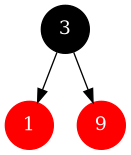
\includegraphics[width=0.85in]{1.png}
%			\caption{insert 9, 3, 1}
		\end{minipage}%
	}%
	\subfigure[]{
		\begin{minipage}[t]{0.25\linewidth}
			\centering
			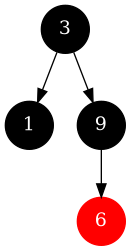
\includegraphics[width=0.82in]{2.png}
%			\caption{insert 6}
		\end{minipage}%
	}%
	\subfigure[]{
	\begin{minipage}[t]{0.3\linewidth}
		\centering
		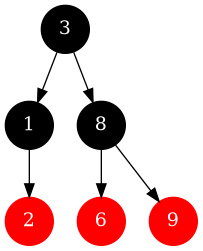
\includegraphics[width=1.3in]{3.png}
		%\caption{fig2}
	\end{minipage}
}%
	%这个回车键很重要 \quad也可以
	
	\subfigure[]{
		\begin{minipage}[t]{0.3\linewidth}
			\centering
			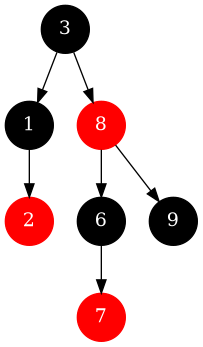
\includegraphics[width=1.3in]{4.png}
			%\caption{fig2}
		\end{minipage}
	}%
	\subfigure[]{
		\begin{minipage}[t]{0.3\linewidth}
			\centering
			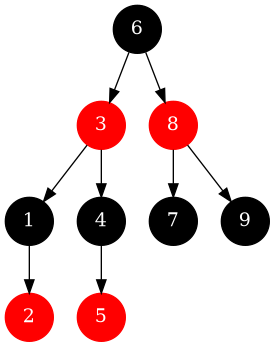
\includegraphics[width=1.8in]{5.png}
			%\caption{fig2}
		\end{minipage}
	}%
	
	\centering
%	\caption{ pics}
\end{figure}


	\end{solution}

\newpage
\item  Show the alphabet trie for the following collection of words: \{chicken, goose, deer, horse, antelope, anteater, goldfish, ant, goat, duck\}.

	\begin{solution} 
	\hspace*{\fill}
		\begin{figure}[ht]
			\centering
			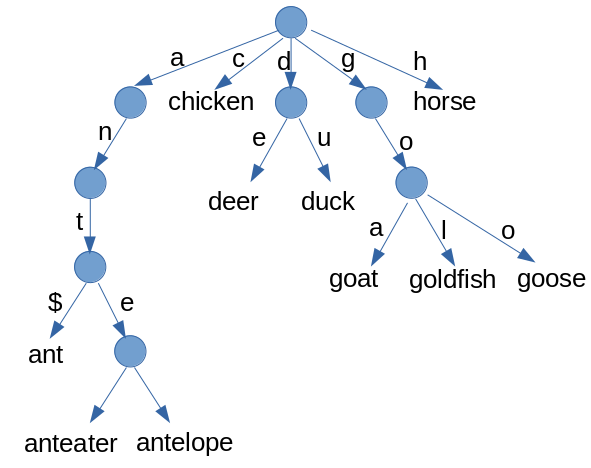
\includegraphics[width=0.9\linewidth]{trie.png}
%			\caption{}
			\label{fig:6}
		\end{figure}
	\end{solution}

\item  Show that any arbitrary n-node binary search tree can be transformed into any other arbitrary n-node binary search tree using $O(n)$ rotations. 

	{\color{blue} Hint: First show that at most $n − 1$ right rotations suffice to transform the tree into a right-skewed binary search tree.}

	\begin{solution} 
		\hspace*{\fill}
		
		a). Each right rotation will increase the length of the rightmost chain by at least 1. Therefore, for an arbitrary n-node BST, in the worst case (the right most chain has only 1 node), it needs $n-1$ right rotations to transform the BST into a right-skewed BST.
		
		b). Suppose we start from $T_1$, and transform $T_1$ into $T_2$. From $T_1$ to right-skewed BST, we need $m$ right rotations, and From $T_2$ to right-skewed BST, we need $k$ right rotations. Since rotation is reversible, we can do $k$ steps of reverse right rotations to transform right-skewed BST to $T_2$. Therefore, in total, we need $m+k < (n-1) + (n-1) = 2n-2 = O(n)$ rotations to transform $T_1$ into $T_2$.
		
		
	\end{solution}

\newpage
\item  Suppose that an AVL tree insertion breaks the AVL balance condition. Suppose node $P$ is the first node that has a balance condition violation in the insertion access path from the leaf. Assume the key is inserted into the left subtree of $P$ and the left child of $P$ is node $A$. Prove the following claims:
	\begin{enumerate}
		\item  Before insertion, the balance factor of node $P$ is 1. After insertion and before applying rotation to fix the violation, the balance factor of node $P$ is 2.
		\item Before insertion, the balance factor of node $A$ is 0. After insertion and before applying rotation to fix the violation, the balance factor of node $A$ cannot be 0.
	\end{enumerate}
	
	\begin{solution} 
				\hspace*{\fill}
		\begin{enumerate}
			\item 
		Suppose before insertion, 
		$B_P = h_{P,l} - h_{P,r}$, $B_A = h_{A,l} - h_{A,r}$,.
		
		After insertion, 
		$B'_P = h'_{P,l} - h'_{P,r}$, $B'_A = h'_{A,l} - h'_{A,r}$.
		 
		Since the key is inserted into the left subtree of $P$, $h'_{P,r} = h_{P,r}$, and $0 \leq h'_{P,l} - h_{P,l} \leq 1$.
		
		Therefore, we have $0 \leq B'_P - B_P \leq 1$, 
		
		Since P is balanced before insertion, $-1 \leq B_P \leq B'_{P} \leq B_P+1 \leq  2$.
		
		But since P is not balanced after insertion, $|B'_P| \geq 2 \Rightarrow B'_P = 2$.
		
		Then $2 \leq B_P + 1 \leq 2 \Rightarrow B_P = 1$ .
		
		\item 
		We have $B_P = h_{P,l} - h_{P,r} = \max\{ h_{A,l}, h_{A,r}\} - h_{P,r}$ = 1.
		
		$B'_P = \max\{ h'_{A,l}, h'_{A,r}\} - h'_{P,r} =\max\{ h'_{A,l}, h'_{A,r}\} - h_{P,r} = 2$.
		
		Therefore, $\max\{ h'_{A,l}, h'_{A,r}\}  = \max\{ h_{A,l}, h_{A,r}\}  + 1$.
		
		Suppose the key is inserted into the left subtree of node $A$:
		
		\qquad Then, $h'_{A,r} = h_{A,r} \Rightarrow \max\{ h'_{A,l}, h_{A,r}\}  = \max\{ h_{A,l}, h_{A,r}\}  + 1$
		
		\qquad If  $h'_{A,l} <  h_{A,r}$
		
		\qquad \qquad then $h_{A,r} = \max\{ h_{A,l}, h_{A,r}\} + 1$ 
		
		\qquad \qquad $\Rightarrow h'_{A,l} < h_{A,r} = h_{A,l} + 1$
		
		\qquad \qquad which is impossible because  the key is inserted into the left subtree of $A$.
				
		\qquad So,   $h'_{A,l} = \max\{ h_{A,l}, h_{A,r}\} + 1$
		
		\qquad So, $h'_{A,l} - h_{A,l} = \max\{ h_{A,l}, h_{A,r}\} - h_{A,l} + 1 \geq 1 \Rightarrow h'_{A,l} - h_{A,l} = 1$ 
		
		\qquad Therefore, $B'_A = B_A + 1 \leq 1$. 
		
		\qquad If $B_A = -1$, then the key must be inserted into the left of node $A$, or it will violate 
		
		\qquad the balance condition.
		
		\qquad Then, $h'_{P,l} =h_{P,l}$, $B'_P = B_P = 1$, which contradicts to what we proved in (a).
		
		\qquad Therefore, $B_A = 0, B'_A = 1$.
		
		Similarly, if the key is inserted into the right  of node $A$, we can  get  $B_A = 0, B'_A = -1$.
		\end{enumerate}
	\end{solution}

\end{enumerate}

%========================================================================
\end{document}